\documentclass[12pt,a4paper]{article}
\usepackage[utf8]{inputenc}
\usepackage[spanish]{babel}
\usepackage{amsmath}
\usepackage{amsfonts}
\usepackage{amssymb}
\usepackage{graphicx}
\usepackage[left=2cm,right=2cm,top=2cm,bottom=2cm]{geometry}
\author{Enciso Guerrero Benjamin Salvador\\
Carlos Enrrique Moran Garabito\\
Cinematica De Robots }
\title{Operador Jacobiano.}
\begin{document}
\maketitle

\includegraphics[scale=1.8]{upzmgg.jpg} 
\newpage
\textbf{Operador Jacobiano.}
\\\\
En calculo vectorial, se llama jacobiano o determinante jacobiano al determinante de la matriz jacobiana. Tanto la matriz jacobiana como el determinante jacobiano reciben su nombre en honor al matemático Carl Gustav Jacobi.
\\\\
La matriz jacobiana es una matriz formada por las derivadas parciales de primer orden de una función. Una de las aplicaciones más interesantes de esta matriz es la posibilidad de aproximar linealmente a la función en un punto. En este sentido, el jacobiano representa la derivada de una función multivariable.
\\\\
\textbf{Función Vectorial.}
\\\\
Supongamos   es una función que va del espacio euclideo n-dimensional a otro espacio euclídeo m-dimensional. Esta función está determinada por m funciones escalares reales:
\\\\
Cuando la función anterior es diferenciable, entonces las derivadas parciales de estas m funciones pueden ser organizadas en una matriz m por n, la matriz jacobiana de F es:
\\\\
Esta matriz es notada de diversas maneras:
\\\\
Nótese que la fila, i-ésima fila coincidirá dada con el gradiente de la función yi, para i = 1,...,m.
\\\\
Si p es un punto de Rn y F es diferenciable en p, entonces su derivada está dada por JF(p). En este caso, la aplicación lineal descrita por JF(p) es la mejor aproximación lineal de F cerca del punto p, de esta manera:
\\\\
Para x cerca de p. O con mayor precisión:
\\\\

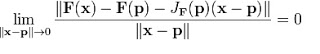
\includegraphics[scale=1]{primera.jpg}
\\\\
Ejemplo. La matriz jacobiana de la función F : R3 -> R3 definida como:
\\\\
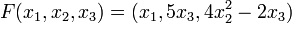
\includegraphics[scale=1]{segunda.jpg} 
\\\\
es:
\\\\
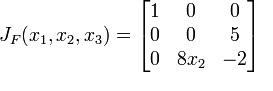
\includegraphics[scale=1]{tercera.jpg}

\end{document}